\documentclass[11pt,a4paper]{article}
\usepackage[T1]{fontenc}
\usepackage[utf8]{inputenc}
\usepackage[indonesian]{babel}
\usepackage[a4paper,margin=23mm]{geometry}
\usepackage{amsmath,booktabs,graphicx,tabularx,float}
\usepackage{tikz}
\usetikzlibrary{arrows.meta,positioning}
\usepackage[hidelinks,hypertexnames=false]{hyperref}
\graphicspath{{figures/}}
\setlength{\parindent}{0pt}
\setlength{\parskip}{5pt}
\renewcommand{\arraystretch}{1.12}
\setcounter{tocdepth}{2}
\tikzset{stage/.style={draw=blue!50!black,fill=blue!5,rounded corners=2pt,
 align=center,minimum height=9mm,font=\small,inner sep=4pt},
 flow/.style={-{Stealth[length=2mm]},thick,draw=blue!55!black}}
\newcommand{\macpair}[2]{\ensuremath{#1\times#2}}
\begin{document}
\raggedbottom
\begin{titlepage}
\centering
\vspace*{28mm}
{\large DRAF LAPORAN PROYEK\par}
\vspace{11mm}
{\huge\bfseries Perancangan dan Evaluasi CNN Integer untuk Klasifikasi Rambu Lalu Lintas pada FPGA Basys 3\par}
\vspace{9mm}
{\large Model 8 dan 43 kelas serta eksperimen paralelisme MAC\par}
\vfill
{\large Tim FPGA Road Sign CNN\par}
\vspace{3mm}
Saufik Ramadhan, Rubi Naufaul, Mahardika, Kania Ika, dan Dika\par
\vspace{12mm}
4 November 2026\par
Snapshot repositori \texttt{ceb5ea86}
\end{titlepage}

\section*{Abstrak}
Proyek ini mengimplementasikan klasifikasi citra rambu GTSRB pada Digilent
Basys 3 menggunakan jaringan saraf konvolusional dengan inferensi integer.
Baseline A dan D42 mengenali delapan kelas dengan akurasi validasi integer
96,63\% dan 97,25\% pada 2.760 citra yang sama. C-43 seed 44 mengenali 43
kelas dan memperoleh 89,60\% pada 12.630 citra uji resmi. Pengujian fisik
mengonfirmasi 23.542 dan 81.168 siklus per citra melalui UART untuk A dan
D42. C-43 cocok dengan referensi integer pada 46 vektor simulasi, dan
uji fisik stored lulus pada 16 slot. Eksperimen baseline A mempertahankan
bobot dan bias sambil mengubah paralelisme Conv1 serta fully connected.
Seluruh kombinasi lulus simulasi, dan sebelas bitstream baru memenuhi
timing 100 MHz. Varian \macpair{9}{8} mencapai 55,73~\(\mu\)s berdasarkan
counter simulasi dan clock build, dengan 18 DSP.

\textbf{Kata kunci} FPGA, Basys 3, GTSRB, CNN integer, kuantisasi, parallel MAC.

\tableofcontents
\listoffigures
\listoftables
\clearpage

\section{Pendahuluan}
Klasifikasi rambu menghadapi variasi pencahayaan, ukuran, dan kemiripan
pola antarkelas. German Traffic Sign Recognition Benchmark (GTSRB)
menyediakan citra berlabel untuk membandingkan metode pada tugas ini
\cite{stallkamp}. Sistem proyek menerima citra satu rambu yang sudah
dipraproses atau membaca bank citra di board, lalu mengeluarkan indeks kelas.

Evaluasi menjawab dua pertanyaan. Bagaimana pilihan arsitektur memengaruhi
akurasi dan kelas yang sering tertukar? Berapa banyak latensi dapat
dikurangi melalui paralelisme pada model yang sama? A dan D42 dibandingkan
pada tugas delapan kelas. C-43 memperluas cakupan ke 43 kelas. Sweep MAC
mengisolasi perubahan hardware dengan mempertahankan paket baseline A.

\section{Dasar Teori}
\subsection{CNN dan keputusan kelas}
Kernel konvolusi dipakai ulang di berbagai posisi spasial. ReLU
membatasi keluaran negatif menjadi nol, dan max pooling mengambil
aktivasi terbesar di setiap jendela. Lapisan fully connected (FC)
menggabungkan \(F\) fitur menjadi satu skor untuk tiap kelas
\cite{goodfellow}.
\[
 z_k=b_k+\sum_{i=0}^{F-1}w_{k,i}a_i,\qquad
 \hat{k}=\operatorname*{arg\,max}_k z_k.
\]
\textit{Max} memberikan nilai terbesar. Argmax memberikan indeks kelasnya.
RTL menyimpan indeks pertama saat dua skor bertanda sama. Softmax
menormalkan skor, tetapi eksponensial dan penyebut positif yang sama
mempertahankan urutan. FPGA cukup memakai komparator untuk menentukan
pemenang tanpa menghitung eksponensial dan pembagian
\cite{goodfellow}.

\subsection{Kuantisasi, MAC, dan timing}
Kuantisasi memungkinkan inferensi dengan operasi integer
\cite{jacob}. Format \texttt{signed24} menyatakan integer bertanda 24 bit
dengan rentang \(-2^{23}\) sampai \(2^{23}-1\). Skala menentukan arti
nilai mentah. Integer 1.200 pada skala 0,01 merepresentasikan 12,0.
Training berjalan dengan floating-point, sedangkan RTL melakukan
aritmetika integer.

MAC mengalikan operand dan menambahkan hasilnya ke akumulator.
Jumlah MAC per citra menggambarkan beban algoritme. Jumlah jalur MAC
membatasi operasi yang dapat dijadwalkan bersamaan. DSP dapat memetakan
operasi aritmetika, sementara BRAM menyimpan bobot atau aktivasi.
Manfaat paralelisme juga bergantung pada bandwidth operand dan routing
\cite{sze}. Setup slack positif menunjukkan bahwa data memenuhi batas
waktu sebelum tepi clock penangkap.

\subsection{Akurasi, recall, dan confusion matrix}
Pada matriks \(C\), baris \(i\) adalah kelas aktual dan kolom \(j\)
adalah prediksi.
\[
 \mathrm{akurasi}=\frac{\sum_i C_{ii}}{\sum_{i,j} C_{ij}},\qquad
 \mathrm{recall}_i=\frac{C_{ii}}{\sum_j C_{ij}}.
\]
Recall makro merupakan rata-rata recall semua kelas. Heatmap
menormalisasi setiap baris menjadi 100\%, sehingga diagonal menunjukkan
recall dan sel lain menunjukkan tujuan salah klasifikasi.

\section{Dataset dan Metode Pelatihan}
GTSRB mencakup 43 kelas \cite{stallkamp}. Split dibuat per track agar
frame dari rangkaian yang sama tidak tersebar di training dan validasi.
A dan D42 memakai 11.130 citra training dan 2.760 citra validasi.
Eksperimen 43 kelas memakai 31.379 citra training dan 7.830 citra
validasi. Official test C-43 memakai 12.630 citra setelah seed 44
dipilih berdasarkan validasi integer.

Pipeline document-v2 memotong ROI dengan koordinat maksimum inklusif,
mengubah citra ke grayscale, melakukan ekualisasi histogram, lalu
mengubah ukuran dengan interpolasi bilinear. Masukan float dibagi 255.
Rotasi ringan, translasi, dan perubahan kecerahan dipakai saat training.
Eksperimen memakai Adam, loss berbobot kelas, dan seed 42, 43, serta 44
\cite{repo}.

\begin{table}[H]
\centering
\caption{Profil arsitektur yang dipertimbangkan.}
\begin{tabular}{llll}
\toprule
Profil & Input & Filter Conv1 & Perubahan desain \\
\midrule
A & $16\times16$ & 8 & Satu Conv dan satu FC \\
B & $32\times32$ & 8 & Resolusi masukan lebih tinggi \\
C & $16\times16$ & 16 & Conv1 lebih lebar \\
D & $16\times16$ & 8 & Conv2 setelah pooling \\
\bottomrule
\end{tabular}
\end{table}

Pada eksperimen 43 kelas, B dan C mencapai rata-rata validasi float
92,12\% dan 92,07\% pada tiga seed. C membutuhkan 61.936 MAC per citra,
dibanding 142.200 pada B. C-43 seed 44 memiliki validasi integer tertinggi
di antara seed C. D42 berasal dari profil D delapan kelas dan dipilih
antara lain karena recall Speed Limit 30 pada validasi. Angka 42 dan
44 menyatakan seed.

\section{Arsitektur Model dan Kuantisasi}
Conv1 menggunakan kernel \(3\times3\) tanpa padding. MaxPool
\(2\times2\) dengan stride 2 menghasilkan ukuran spasial \(7\times7\).
Conv2 D42 memakai padding nol satu piksel dan membaca delapan channel
masukan untuk setiap filter keluaran. Satu output Conv2 membutuhkan
72 perkalian. A dan D42 meratakan 392 fitur, sedangkan C-43
meratakan 784 fitur dalam urutan CHW.

\begin{figure}[H]
\centering
\begin{tikzpicture}[node distance=3mm]
\node[stage] (a1) {A\\$1\times16\times16$};
\node[stage,right=of a1] (a2) {Conv1\\$8\times14\times14$};
\node[stage,right=of a2] (a3) {MaxPool\\$8\times7\times7$};
\node[stage,right=of a3] (a4) {Flatten\\392 fitur};
\node[stage,right=of a4] (a5) {FC\\8 skor};
\node[stage,below=6mm of a1] (d1) {D42\\$1\times16\times16$};
\node[stage,right=of d1] (d2) {Conv1\\$8\times14\times14$};
\node[stage,right=of d2] (d3) {MaxPool\\$8\times7\times7$};
\node[stage,right=of d3] (d4) {Conv2\\$8\times7\times7$};
\node[stage,right=of d4] (d5) {Flatten\\392 fitur};
\node[stage,right=of d5] (d6) {FC\\8 skor};
\node[stage,below=6mm of d1] (c1) {C-43\\$1\times16\times16$};
\node[stage,right=of c1] (c2) {Conv1\\$16\times14\times14$};
\node[stage,right=of c2] (c3) {MaxPool\\$16\times7\times7$};
\node[stage,right=of c3] (c4) {Flatten\\784 fitur};
\node[stage,right=of c4] (c5) {FC\\43 skor};
\foreach \u/\v in {a1/a2,a2/a3,a3/a4,a4/a5,d1/d2,d2/d3,d3/d4,d4/d5,d5/d6,c1/c2,c2/c3,c3/c4,c4/c5}
  \draw[flow] (\u)--(\v);
\end{tikzpicture}
\caption{Aliran tensor dalam urutan channel, tinggi, lebar. Setiap Conv diikuti requantization dan ReLU. Argmax mengambil indeks skor FC terbesar.}
\end{figure}

\begin{table}[H]
\centering
\caption{Jumlah parameter dan MAC nominal per citra. Hitungan Conv2 mencakup tap padding.}
\begin{tabular}{lrrrrrr}
\toprule
Model & Bobot & Bias & MAC Conv1 & MAC Conv2 & MAC FC & Total MAC \\
\midrule
A & 3.208 & 16 & 14.112 & 0 & 3.136 & 17.248 \\
D42 & 3.784 & 24 & 14.112 & 28.224 & 3.136 & 45.472 \\
C-43 & 33.856 & 59 & 28.224 & 0 & 33.712 & 61.936 \\
\bottomrule
\end{tabular}
\end{table}

Bobot memakai int8, piksel uint8, dan bias, accumulator serta skor
signed24. Requantization mengubah skala keluaran Conv dan membatasi
aktivasi ke 0--127. Untuk accumulator \(a\) dan \(S>0\), RTL menghitung
\[
 q=\min\left(127,\left\lfloor
 \frac{\max(0,a)M+2^{S-1}}{2^S}
 \right\rfloor\right).
\]
A memakai \((M,S)=(43980,25)\). D42 memakai \((53859,26)\) pada Conv1
dan \((54743,24)\) pada Conv2. C-43 seed 44 memakai \((38660,24)\).
Kalibrasi memakai citra training. Batas konservatif jumlah antara
adalah \(|b|+a_{\max}\sum_i|w_i|\). Batas terbesar dari tiga seed C-43
yang dikuantisasi adalah 835.898, di bawah 8.388.607. RTL memeriksa
overflow pada tiap penjumlahan, termasuk bila overflow kemudian
terkompensasi. Paket model memuat parameter, kontrak, golden dan
checksum \cite{repo}.

\section{Implementasi RTL pada Basys 3}
\begin{figure}[H]
\centering
\begin{tikzpicture}[node distance=4mm]
\node[stage] (in) {ROM stored\\atau RAM LIVE};
\node[stage,right=of in] (cv) {Conv1 +\\requant};
\node[stage,right=of cv] (ram) {RAM\\fitur};
\node[stage,right=of ram] (pool) {MaxPool\\+ RAM};
\node[stage,right=of pool] (fc) {FC\\dan argmax};
\node[stage,below=5mm of pool] (conv2) {Conv2 + requant\\khusus D42};
\node[stage,right=of fc] (out) {Display\\atau UART};
\draw[flow] (in)--(cv); \draw[flow] (cv)--(ram);
\draw[flow] (ram)--(pool); \draw[flow] (pool)--(fc);
\draw[flow] (pool)--(conv2); \draw[flow] (conv2.east)-|(fc.south);
\draw[flow] (fc)--(out);
\end{tikzpicture}
\caption{Datapath sistem. D42 meneruskan keluaran pooling melalui Conv2 sebelum FC. A dan C-43 meneruskannya langsung ke FC.}
\end{figure}

A dan D42 menerima input LIVE melalui UART 115200 8N1. Request berukuran
259 byte dan reply 32 byte, termasuk delapan skor signed24 dan counter
siklus 32 bit. Untuk stored, SW3--SW0 memilih citra, SW15 diset rendah,
dan BTNC memicu inferensi. C-43 menggunakan 16 citra stored, indeks
6 bit, dan dua digit desimal. UART pada profil ini idle. Model Studio
memilih arsip dan memverifikasi checksum sebelum pemrograman JTAG
\cite{repo}.

\subsection{Penjadwalan Conv dan FC}
Conv1 serial menerima satu tap per siklus setelah pipeline terisi.
Varian 3 dan 9 MAC membentuk jendela \(3\times3\) melalui line buffer
dan memproses satu baris kernel atau satu kernel per langkah
\cite{pr8}. FC paralel membagi kelas ke bank bobot dan membagikan satu
aktivasi ke semua jalur. Setiap jalur menjaga urutan MAC per kelas,
dan posisi skor pada bus tetap mengikuti indeks kelas.

\begin{figure}[H]
\centering
\begin{tikzpicture}[node distance=8mm]
\node[stage] (idle) {IDLE};
\node[stage,right=of idle] (issue) {ISSUE};
\node[stage,right=of issue] (mac) {MAC};
\node[stage,right=of mac] (scale) {SCALE};
\node[stage,right=of scale] (wait) {WAIT\_Q};
\draw[flow] (idle)--(issue);
\draw[flow] (issue)--(mac);
\draw[flow] (mac)--(scale);
\draw[flow] (scale)--(wait);
\draw[flow] (mac) to[bend right=55] node[above,font=\scriptsize]{tap berikutnya} (issue);
\draw[flow] (wait) to[bend left=22] node[below,font=\scriptsize]{tulis aktivasi, lanjut output} (issue);
\draw[flow] (wait) to[bend left=44] node[below,font=\scriptsize]{output terakhir, done} (idle);
\end{tikzpicture}
\caption{FSM Conv2 D42. Setelah tap ke-72, SCALE mengirim accumulator ke requantizer. WAIT\_Q menunggu hasil valid sebelum menulis aktivasi.}
\end{figure}

\subsection{Jalur kritis C-43}
ROM bobot FC dipetakan ke BRAM. Percobaan 100 MHz gagal setup pada jalur
BRAM bobot ke register skor dengan slack \(-2{,}109\) ns. Bitstream
terpasang menggunakan core 50 MHz dari clock board 100 MHz, dengan setup
slack \(+4{,}658\) ns dan hold slack \(+0{,}069\) ns. Pada build 50 MHz,
delay jalur terburuk adalah 14,88 ns, terdiri dari 7,20 ns logika dan
7,68 ns routing. Penempatan dan routing build 50 MHz berbeda dari
percobaan 100 MHz \cite{repo}.

\section{Metode Verifikasi dan Pengukuran}
Model Python integer menjadi referensi untuk RTL. Testbench
membandingkan tensor antara sesuai cakupan tiap tes, skor bertanda,
prediksi, flag overflow, dan jumlah siklus. Vivado melaporkan
penggunaan LUT, FF, BRAM serta DSP, slack setup dan hold, dan hasil DRC.

Latensi core dihitung dengan \(t=N/f\), dengan \(N\) jumlah siklus
dan \(f\) frekuensi clock. A dan D42 memakai counter RTL yang dibaca
dari reply UART pada board fisik. Untuk C-43, \(N\) diukur dalam
simulasi datapath dari start Conv hingga done argmax. Varian MAC baru
juga memakai counter simulasi dan frekuensi hasil build. Round-trip UART
mencakup transfer serial serta penjadwalan host, sehingga dicatat
terpisah dari latensi komputasi.

\section{Hasil dan Pembahasan}
\subsection{Validasi delapan kelas}
A seed 42 mencapai 96,92\% pada float dan 96,63\% pada integer.
D42 mencapai 97,28\% pada float dan 97,25\% pada integer. Selisih
integer 0,62 poin persentase merupakan hasil deskriptif untuk dua
checkpoint. Recall makro integer masing-masing 97,08\% dan 97,75\%.

\begin{table}[H]
\centering
\caption{Recall per kelas pada validasi 2.760 citra.}
\begin{tabular}{rrlrr}
\toprule
Indeks RTL & ID GTSRB & Kelas & A (\%) & D42 (\%) \\
\midrule
0 & 14 & Stop & 98,00 & 100,00 \\
1 & 13 & Yield & 99,52 & 99,76 \\
2 & 17 & No entry & 98,57 & 99,52 \\
3 & 12 & Priority road & 98,57 & 98,33 \\
4 & 18 & General caution & 99,17 & 98,75 \\
5 & 38 & Keep right & 98,81 & 98,33 \\
6 & 1 & Speed limit 30 & 85,56 & 93,11 \\
7 & 2 & Speed limit 50 & 98,44 & 94,22 \\
\bottomrule
\end{tabular}
\end{table}

\begin{figure}[H]
\centering
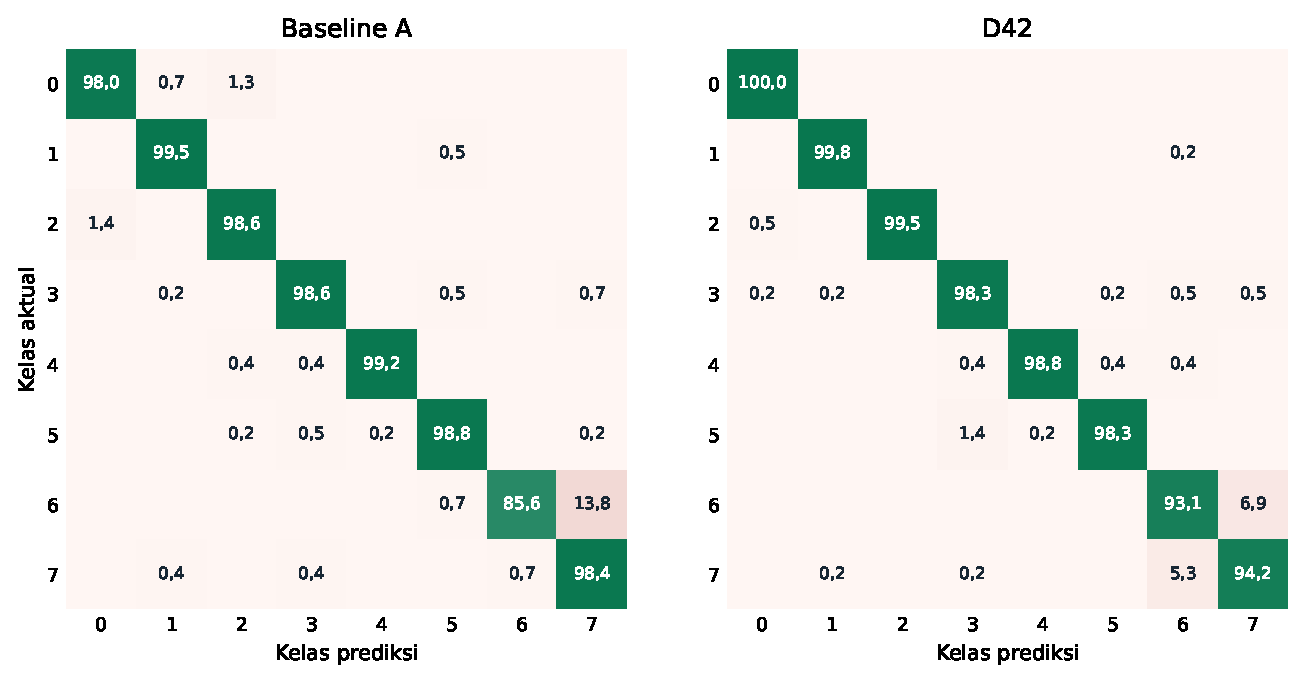
\includegraphics[width=\linewidth]{validasi-8-kelas.pdf}
\caption{Heatmap validasi delapan kelas. Hijau menandai prediksi benar dan merah menandai kesalahan. Kedua panel memakai skala 0--100\% per baris. Sel tanpa angka bernilai nol.}
\end{figure}

Recall Speed Limit 30 naik dari 85,56\% ke 93,11\%. Perubahan ini lebih
besar dari kenaikan akurasi keseluruhan. Official test A dan D42 masih
terbuka. Semua varian MAC A memakai parameter yang sama dan cocok
dengan golden pada vektor simulasi. Heatmap A mewakili model yang
digunakan oleh semua varian tersebut.

\subsection{Official test C-43 seed 44}
\begin{table}[H]
\centering
\caption{Perbandingan float dan integer C-43 seed 44.}
\begin{tabular}{llrr}
\toprule
Set & Model & Akurasi (\%) & Total citra \\
\midrule
Validasi & Float & 92,49 & 7.830 \\
Validasi & Integer & 92,52 & 7.830 \\
Official test & Float & 89,56 & 12.630 \\
Official test & Integer & 89,60 & 12.630 \\
\bottomrule
\end{tabular}
\end{table}

Recall makro official test adalah 86,40\% pada float dan 86,52\%
pada integer. C-43 integer menjawab benar 11.317 citra, enam lebih
banyak dari float, walaupun 202 prediksi berubah. Akurasi integer
turun 2,92 poin persentase dari validasi ke official test. Cakupan
kelas dan set evaluasinya berbeda dari perbandingan A dan D42.

\begin{figure}[H]
\centering
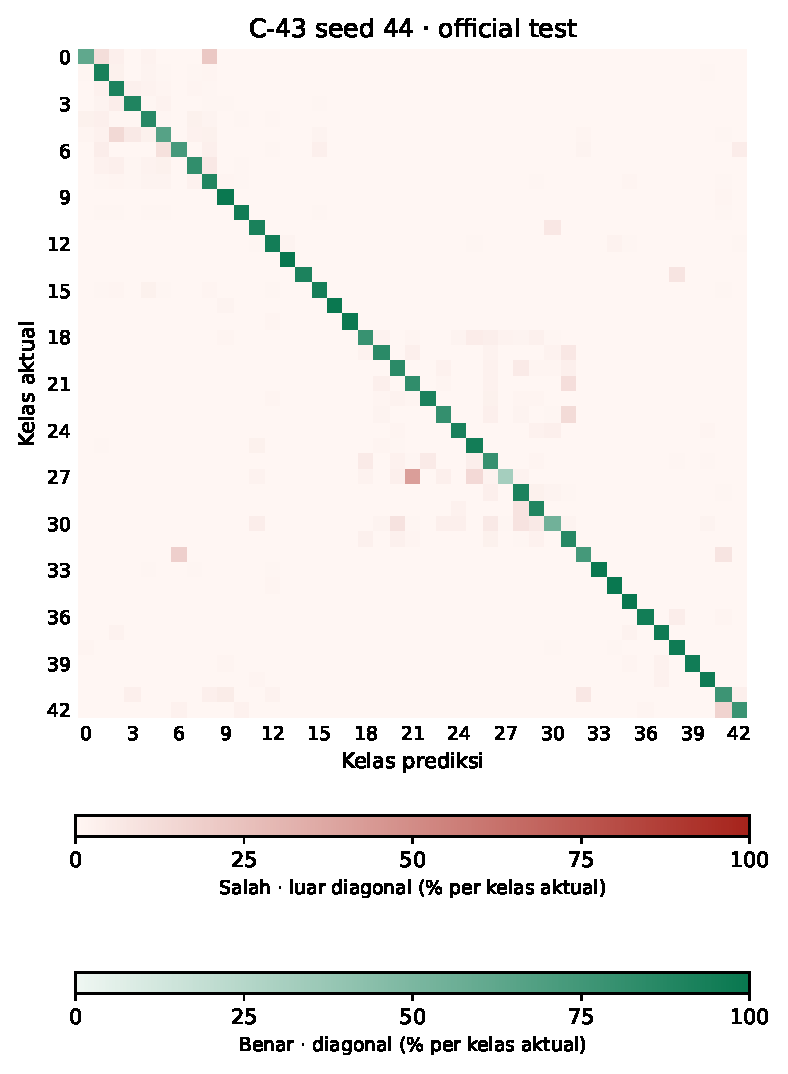
\includegraphics[width=.75\linewidth]{official-c43.pdf}
\caption{Heatmap official test C-43 integer. Sumbu memakai ID GTSRB 0--42. Warna menunjukkan persentase terhadap jumlah citra per kelas aktual.}
\end{figure}

\begin{figure}[H]
\centering
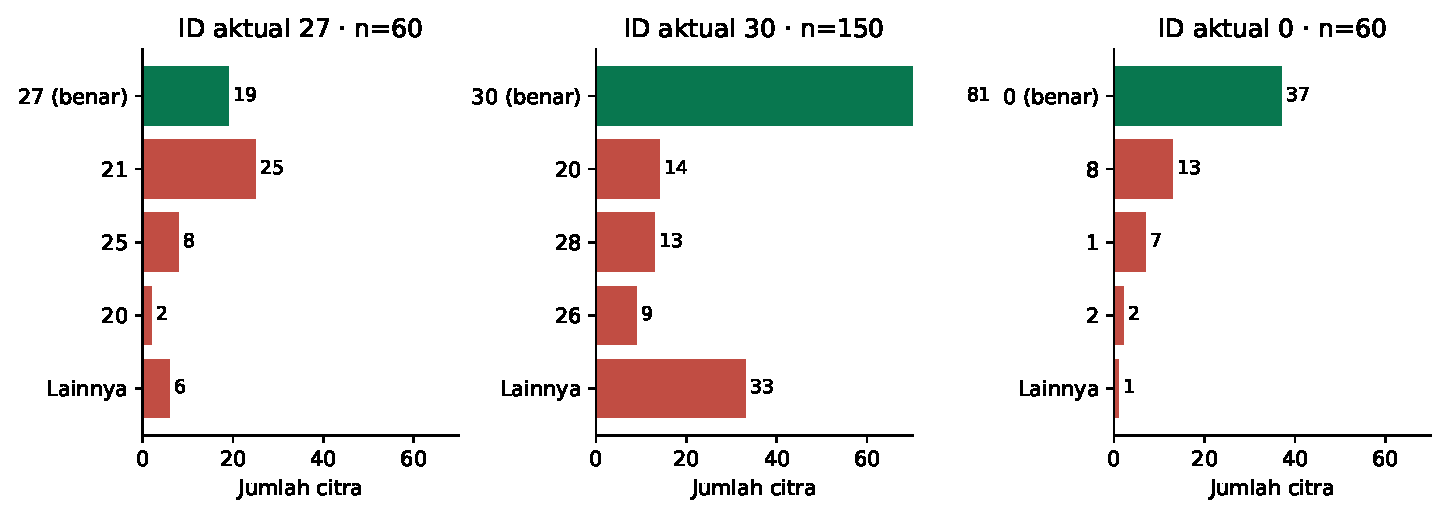
\includegraphics[width=\linewidth]{detail-c43.pdf}
\caption{Tiga kelas dengan recall terendah. Hijau menunjukkan jumlah prediksi benar. Merah menunjukkan tiga tujuan salah prediksi terbesar dan agregat kesalahan lainnya.}
\end{figure}

ID 27 (pejalan kaki) dikenali pada 19 dari 60 citra. Sebanyak 25 citra kelas ini
diprediksi sebagai ID 21. ID 30 dikenali pada 81 dari 150 citra,
dengan salah prediksi terbanyak menuju ID 20 dan 28. ID 0 dikenali
pada 37 dari 60 citra, dengan 13 prediksi menuju ID 8. Ketiga recall
tersebut adalah 31,67\%, 54,00\%, dan 61,67\%.

\subsection{Latensi dan resource FPGA}
\begin{table}[H]
\centering\small
\caption{Latensi core dan resource pasca-routing. Resource A dan D42 berasal dari build PR \#7.}
\begin{tabular}{lrrrrrrrr}
\toprule
Model & MHz & Siklus & $\mu$s & LUT & FF & BRAM & DSP & WNS (ns) \\
\midrule
A & 100 & 23.542 & 235,42 & 1.106 & 934 & 2,5 & 3 & +0,980 \\
D42 & 100 & 81.168 & 811,68 & 1.331 & 1.004 & 3 & 5 & +0,845 \\
C-43 & 50 & 101.970 & 2.039,40 & 1.720 & 1.362 & 19 & 4 & +4,658 \\
\bottomrule
\end{tabular}
\end{table}

Conv2 serial mendominasi kenaikan siklus D42. FC C-43 membutuhkan
33.712 MAC per citra dengan satu jalur serial. Clock 50 MHz membuat
siklusnya dua kali lebih lama daripada clock 100 MHz. C-43 memakai
38\% dari 50 BRAM tile. Latensi 2,04 ms dihitung dari simulasi datapath.
Counter fisik C-43 belum diukur. Median round-trip UART A dan D42
sekitar 31,92 ms pada pengujian masing-masing \cite{repo}.

\subsection{Sweep 12 kombinasi MAC baseline A}
\begin{table}[H]
\centering\small
\caption{Kombinasi Conv1 dan FC pada 100 MHz. Latensi dihitung dari counter RTL. Setup dan hold dalam ns.}
\begin{tabular}{rrrrrrrrr}
\toprule
Conv1 $\times$ FC & Siklus & $\mu$s & LUT & FF & BRAM & DSP & Setup & Hold \\
\midrule
1 $\times$ 1 & 23.542 & 235,42 & 1.106 & 934 & 2,5 & 3 & +0,980 & +0,040 \\
1 $\times$ 2 & 20.406 & 204,06 & 1.147 & 972 & 2,5 & 4 & +1,049 & +0,058 \\
1 $\times$ 4 & 18.838 & 188,38 & 1.264 & 1.048 & 2,5 & 6 & +1,152 & +0,034 \\
1 $\times$ 8 & 18.054 & 180,54 & 1.508 & 1.200 & 2,5 & 10 & +0,977 & +0,109 \\
3 $\times$ 1 & 14.195 & 141,95 & 1.235 & 1.015 & 2,5 & 5 & +1,151 & +0,037 \\
3 $\times$ 2 & 11.059 & 110,59 & 1.270 & 1.053 & 2,5 & 6 & +1,182 & +0,056 \\
3 $\times$ 4 & 9.491 & 94,91 & 1.389 & 1.129 & 2,5 & 8 & +1,035 & +0,056 \\
3 $\times$ 8 & 8.707 & 87,07 & 1.631 & 1.281 & 2,5 & 12 & +0,726 & +0,051 \\
9 $\times$ 1 & 11.061 & 110,61 & 1.233 & 1.015 & 2,5 & 11 & +1,137 & +0,059 \\
9 $\times$ 2 & 7.925 & 79,25 & 1.273 & 1.053 & 2,5 & 12 & +1,216 & +0,025 \\
9 $\times$ 4 & 6.357 & 63,57 & 1.390 & 1.129 & 2,5 & 14 & +1,030 & +0,040 \\
9 $\times$ 8 & 5.573 & 55,73 & 1.632 & 1.281 & 2,5 & 18 & +0,835 & +0,034 \\
\bottomrule
\end{tabular}
\end{table}

\begin{figure}[H]
\centering
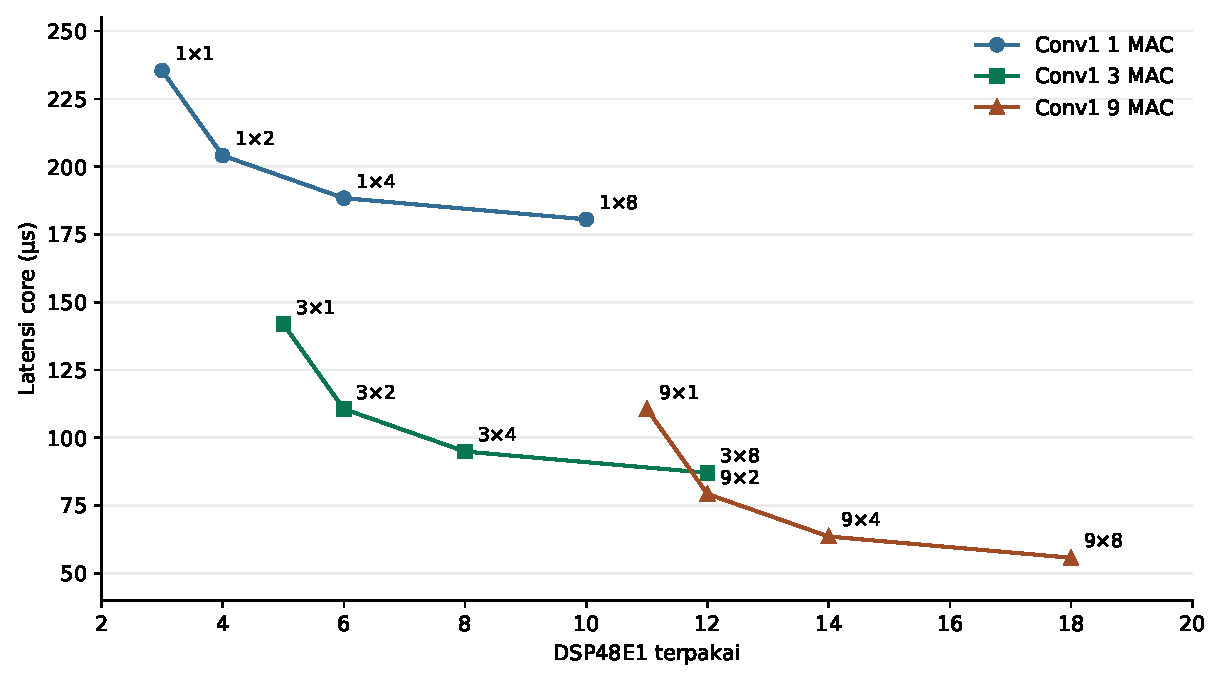
\includegraphics[width=.94\linewidth]{latensi-dsp.pdf}
\caption{Trade-off latensi core dan DSP. Label titik menunjukkan jumlah jalur Conv1 dan FC.}
\end{figure}

Kombinasi \macpair{3}{2} mencapai 110,59~\(\mu\)s dengan enam DSP,
sedangkan \macpair{9}{1} mencapai 110,61~\(\mu\)s dengan sebelas DSP.
Penghematan FC pada varian pertama mengimbangi penghematan Conv1 pada
varian kedua. Kombinasi \macpair{9}{8} mencapai 55,73~\(\mu\)s dengan
18 DSP, atau 4,22 kali lebih cepat dari kontrol. Sebelas build baru
memenuhi setup dan hold pada 100 MHz. Uji fisik varian baru masih
terbuka \cite{repo}.

\subsection{Cakupan verifikasi fisik}
\begin{table}[H]
\centering
\caption{Bukti fisik dan status simulasi tiap konfigurasi.}
\begin{tabularx}{\linewidth}{lXX}
\toprule
Model & LIVE UART & Stored \\
\midrule
A & 304 inferensi valid, 2.432 skor cocok dengan golden & 16/16 slot lulus fisik \\
D42 & 253 inferensi valid, 2.024 skor cocok dengan golden & Lulus simulasi \\
C-43 & UART idle pada profil ini & 16/16 slot lulus fisik \\
MAC A baru & Lulus simulasi top & Lulus simulasi top \\
\bottomrule
\end{tabularx}
\end{table}

Uji LIVE memakai pengulangan vektor dan skenario pemulihan komunikasi.
Kecocokan golden menguji kesetaraan aritmetika dan jalur data untuk
input yang diperiksa. Akurasi terhadap label berasal dari evaluasi
dataset. Uji stored fisik memeriksa display untuk bank citra yang
dipilih. Simulasi datapath C-43 juga memeriksa 46 vektor dan
1.978 skor FC secara bit-exact.

\section{Kesimpulan dan Pekerjaan Lanjutan}
D42 menaikkan akurasi validasi serta recall Speed Limit 30 dengan
tambahan waktu Conv2 serial. C-43 memperluas cakupan menjadi 43 kelas
dan mencapai 89,60\% pada official test, dengan variasi recall yang
besar antarkelas. Sweep MAC menunjukkan bahwa alokasi DSP antara Conv1
dan FC menentukan latensi, bahkan ketika model dan beban MAC nominal
tetap sama.

Pekerjaan terbuka mencakup official test A dan D42, uji fisik stored
D42 dan varian MAC baru, serta evaluasi pipeline penulisan skor FC
C-43 untuk target 100 MHz. LIVE UART C-43 bergantung pada kebutuhan
demo dan format reply yang disepakati.

\appendix
\section{Pemetaan kelas dan data matriks}
Pemetaan indeks RTL A dan D42 ke ID dan nama rambu tercantum pada
tabel recall. C-43 memakai ID GTSRB langsung. Berkas sumber menyertakan
tiga matriks jumlah citra di folder \texttt{data/}. Sumbu A dan D42
mengikuti indeks RTL 0--7. Sumbu C-43 mengikuti ID 0--42.


\begin{table}[H]
\centering\small
\caption{Pemetaan 43 kelas GTSRB. Nama rambu diterjemahkan dari daftar kelas \cite{celen}.}
\begin{tabularx}{\linewidth}{rXrX}
\toprule
ID & Nama rambu & ID & Nama rambu \\
\midrule
0 & Batas 20 km/jam & 22 & Jalan bergelombang \\
1 & Batas 30 km/jam & 23 & Jalan licin \\
2 & Batas 50 km/jam & 24 & Penyempitan dari kanan \\
3 & Batas 60 km/jam & 25 & Pekerjaan jalan \\
4 & Batas 70 km/jam & 26 & Lampu lalu lintas \\
5 & Batas 80 km/jam & 27 & Pejalan kaki \\
6 & Akhir batas 80 km/jam & 28 & Anak menyeberang \\
7 & Batas 100 km/jam & 29 & Pesepeda menyeberang \\
8 & Batas 120 km/jam & 30 & Waspada es atau salju \\
9 & Dilarang mendahului & 31 & Satwa liar menyeberang \\
10 & Larangan mendahului bagi kendaraan berat & 32 & Akhir pembatasan kecepatan dan mendahului \\
11 & Hak jalan di persimpangan & 33 & Belok kanan \\
12 & Jalan prioritas & 34 & Belok kiri \\
13 & Beri jalan & 35 & Wajib lurus \\
14 & Berhenti & 36 & Lurus atau kanan \\
15 & Dilarang masuk semua kendaraan & 37 & Lurus atau kiri \\
16 & Larangan kendaraan di atas 3,5 ton & 38 & Tetap di kanan \\
17 & Dilarang masuk & 39 & Tetap di kiri \\
18 & Peringatan umum & 40 & Wajib mengikuti bundaran \\
19 & Tikungan kiri & 41 & Akhir larangan mendahului \\
20 & Tikungan kanan & 42 & Akhir larangan mendahului bagi kendaraan berat \\
21 & Tikungan ganda &  &  \\
\bottomrule
\end{tabularx}
\end{table}

\section{Reproduksi dan identitas build}
Perintah berikut dijalankan dari root proyek dengan Python 3.11,
Icarus Verilog, dan Vivado 2026.1. Model Studio menyimpan checksum
paket dan bitstream di \texttt{profiles.json}. Salinan identitas
deployment disertakan dalam \path{data/identitas-bitstream.json}.
\begin{verbatim}
python scripts/check_workspace.py --full-model --vivado
python tests/run_rtl_tests.py
python tests/rtl/integration/run_integration_tests.py --mac 3 2
vivado -mode batch -source scripts/build_basys3.tcl -tclargs a-mac 3 2
python apps/model_studio/studio.py
\end{verbatim}

\begin{table}[H]
\centering\small
\caption{Commit sumber bitstream dan pola tag rollback lokal.}
\begin{tabular}{lll}
\toprule
Bitstream & Commit & Tag lokal \\
\midrule
A kontrol & \texttt{3a3074cc} & \texttt{fpga/a-int24-v2/conv1-mac1-fc-mac1} \\
D42 & \texttt{c6902cae} & \texttt{fpga/d42-int24-v1/conv1-mac1-fc-mac1} \\
C-43 & \texttt{bf682e5a} & \texttt{fpga/c43-s44-int24-v1/conv1-mac1-fc-mac1} \\
Sweep A & \texttt{b96c8bd3} & \texttt{fpga/a-int24-v2/conv1-macN-fc-macM} \\
\bottomrule
\end{tabular}
\end{table}

Detail evaluator C-43, parameter per seed, dan hasil build dicatat di
\path{reference_model/results/README.md}, \texttt{tests/README.md},
dan \texttt{docs/HARDWARE.md}. Dataset, checkpoint, serta bitstream
berada di penyimpanan lokal proyek \cite{repo}.

\begin{thebibliography}{9}
\bibitem{stallkamp}
J. Stallkamp, M. Schlipsing, J. Salmen, dan C. Igel,
Man vs. computer: Benchmarking machine learning algorithms for traffic sign recognition.
\textit{Neural Networks}, vol. 32, hlm. 323--332, 2012.
\href{https://doi.org/10.1016/j.neunet.2012.02.016}{doi:10.1016/j.neunet.2012.02.016}.

\bibitem{goodfellow}
I. Goodfellow, Y. Bengio, dan A. Courville, \textit{Deep Learning}.
MIT Press, 2016, bab 6 dan 9.
\url{https://www.deeplearningbook.org/}.

\bibitem{jacob}
B. Jacob dkk., Quantization and Training of Neural Networks for Efficient Integer-Arithmetic-Only Inference.
\textit{Proceedings of the IEEE Conference on Computer Vision and Pattern Recognition}, hlm. 2704--2713, 2018.
\href{https://doi.org/10.1109/CVPR.2018.00286}{doi:10.1109/CVPR.2018.00286}.

\bibitem{sze}
V. Sze, Y.-H. Chen, T.-J. Yang, dan J. S. Emer,
Efficient Processing of Deep Neural Networks: A Tutorial and Survey.
\textit{Proceedings of the IEEE}, vol. 105, no. 12, hlm. 2295--2329, 2017.
\href{https://doi.org/10.1109/JPROC.2017.2761740}{doi:10.1109/JPROC.2017.2761740}.

\bibitem{celen}
A. E. Celen, \textit{Tiny Machine Learning for Embedded Systems: Real-Time Traffic Sign Recognition on Microcontrollers}.
Tugas akhir sarjana, Delft University of Technology, 2025, Lampiran A.
\href{https://repository.tudelft.nl/file/File_c9c48f2c-fd1d-4989-a3b2-2f12265c3bee}{Naskah TU Delft}.

\bibitem{repo}
Tim FPGA Road Sign CNN, \textit{Dokumentasi implementasi, hasil model, dan pengujian}, snapshot \texttt{ceb5ea86}.
\href{https://github.com/saufik-ramadhan/fpga_road_sign_cnn/tree/ceb5ea86}{Repositori proyek}.

\bibitem{pr8}
Mahardika, \textit{P3: 3- and 9-multiplier convolution behind N\_MAC}, 2026.
\href{https://github.com/saufik-ramadhan/fpga_road_sign_cnn/pull/8}{PR \#8 dan catatan simulasi P3}.
\end{thebibliography}
\end{document}
